\documentclass[a4paper,12pt]{article}
\usepackage[left=2.5cm,right=2.5cm,top=2.5cm,bottom=2.5cm]{geometry} 
\usepackage{color}
\usepackage[usenames,dvipsnames]{xcolor}
\usepackage{amsmath,amssymb,amsthm,algorithm,algorithmic,graphicx,yhmath,url,enumitem,lscape,mathtools}
\usepackage{wrapfig,subfigure}

\newcounter{problem}
\newenvironment{problem}{\refstepcounter{problem} \noindent {\bf Problem \arabic{problem}}}{\newpage}
\newenvironment{solution}{\vspace{0.3cm} \par \noindent {\bf Solution}}{}
\newenvironment{verification}{\vspace{0.3cm} \par \noindent {\bf Verification}}{}
\newenvironment{hint}{\vspace{0.3cm} \par {\bf Hint:}}{}

\newcounter{remark}
\newenvironment{remark}{\refstepcounter{remark} \vspace{0.3cm} \par \noindent {\bf Remark \arabic{remark}}}{\vspace{0.3cm}}
\newcounter{lesson}
\newenvironment{lesson}{\refstepcounter{lesson} \vspace{0.3cm} \par \noindent {\bf Lesson \arabic{lesson}}}{\vspace{0.3cm}}
\newcommand{\R}{\mathbb{R}}
\newcommand{\N}{\mathbb{N}}
\newcommand{\Rn}{\mathbb{R}^n}
\newcommand{\Rnn}{\mathbb{R}^{n \times n}}
\newcommand{\bes}{\begin{equation*}}
\newcommand{\ees}{\end{equation*}}
\newcommand{\be}{\begin{equation}}
\newcommand{\ee}{\end{equation}}
\newcommand{\eps}{\epsilon}
\newcommand{\fl}{\text{fl}}

\begin{document}

\title{5DV005, Fall 2018, Lab session 1}
\author{Carl Christian Kjelgaard Mikkelsen}

\maketitle
\tableofcontents

\section{The time and the place}
Our first lab session will take place on
\begin{center}
Wednesday, November 7st, 2018, (kl. 13.00-16.00), Room MA416-426.
\end{center}

\section{Setting the MATLAB path correctly}

\begin{enumerate}
\item Change directory to {\tt 5dv005ht18} and launch {\tt MATLAB} using the command {\tt matlab \&}.
\item Update {\tt MATLAB}'s search path to include the folders
\begin{verbatim}
  5dv005ht18/matlab 
  5dv005ht18/exercises
\end{verbatim}
and all their subfolders. Save the path definition into the file {\tt 5dv005ht18/pathdef.m}
\end{enumerate}
Always launch {\tt MATLAB} from the directory {\tt 5dv005ht18}. This ensures that the search path is set correctly for each session.

\newpage
\section{The problems}

\begin{problem} Within {\tt MATLAB} do:
  \begin{enumerate}
  \item Issue the command {\tt help bal}. This prints a summary of the {\tt MATLAB} files contained in the folder {\tt bal}. These files are for solving problems in external ballistics, i.e. fire control of artillery.
  \item Issue the command {\tt help range\_rk1} and read through the documentation in detail.
  \item Execute the minimal working example {\tt range\_rk1\_MWE1}.
  \end{enumerate} 

  \begin{remark} The function {\tt range\_rk1} demonstrates the standard that is  expect from you! In particular, all your codes must contain the call sequence, a complete description of all input and output variables, as well as a minimal working example. Moreover, all code must contain frequent and helpful comments. Software which does not adhere to this standard will not be accepted.
  \end{remark}
\end{problem}

\begin{problem}
  Copy the script {\tt lab1/scripts/l1p2.m} into {\tt lab1/work/my\_l1p2.m}. Your task is to modify {\tt my\_l1p2.m} so that it produces the output shown in Figure \ref{fig:output} and renders the graphics shown in Figure \ref{fig:trajectories}. These are the {\tt MATLAB} commands which you will need: {\tt fprintf}, {\tt plot}, {\tt axis equal}, {\tt xlabel}, {\tt ylabel}, {\tt grid}, {\tt axis}, {\tt print}.
  
\begin{figure}[ht]
  \begin{verbatim}
                  Flag    Range (meters)     TOI (seconds)
                    1        16844.662          66.33
                    1        14998.963          81.57
\end{verbatim} \caption{The output of {\tt l1p2} after completion.} \label{fig:output}
\end{figure}

\begin{figure}[ht]
\centering
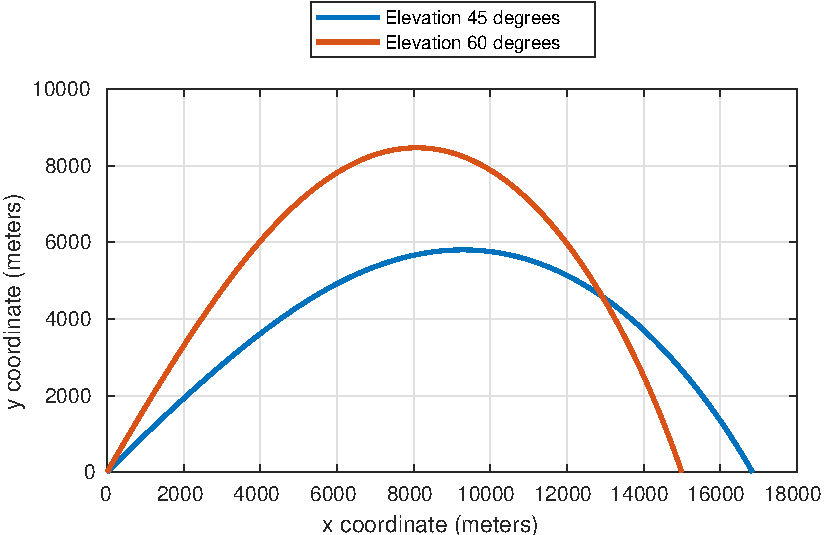
\includegraphics[width=16cm]{fig1.pdf} \caption{The trajectory of a two shells fired at using elevations of 45 degrees and 60 degrees} \label{fig:trajectories}
\end{figure}

\begin{remark}
  In general, I recommend that you export figures from MATLAB at {\tt .eps} files. You can convert the file {\tt fig.eps} to {\tt .pdf} format using the command {\tt ps2pdf -DEPSCrop fig.ps}. This crops the white space and produces a file called {\tt fig.pdf}. 
\end{remark}

\end{problem}

\begin{problem} As demonstrated during yesterday's lecture the problem of computing a sum of positive numbers
  \bes
  s = \sum_{i=1}^m a_i
  \ees
  is substantially more complicated than it would appear! This exercise illustrates highlights the problem and shows how calculate an upper bound for the error.
  \begin{enumerate}  
  \item Copy the script {\tt lab1/scripts/l1p3.m} to {\tt lab1/work/my\_l1p3.m}.
  \item Edit {\tt my\_l1p3} so that it uses {\tt simple\_sum} to compute
    \bes
    s = \sum_{i=1}^m \frac{1}{i}, \quad m = 2^{22}
    \ees
    using single/double precision and ascending/descending order, a total of 4 different calculations.
  \item Edit {\tt my\_l1p3} so that compute the error associated with each value of $s$. An exceedingly accurate value of the true sum $s$ can be obtained using double precision and the function {\tt kahan\_sum}.
  \item Copy function {\tt simple\_sum} to {\tt lab1/work/my\_simple\_sum}.
  \item Edit {\tt my\_simple\_sum} to include the computation of a number $\mu$, such that
    \bes
    |s - \hat{s}| \leq \mu u
    \ees
    where $s$ is the true value of the sum, $\hat{s}$ is computed value of $s$ and $u$ is the unit roundoff. The upper bound, i.e., the term $\mu u$ is called an running error bound, because it is computed concurrently with $s$.
  \item Edit {\tt my\_l1p3} so that it displays the running error bound right next to the actual error.
  \item Verify that the absolute value of the error is bounded by the running error bound.
  \item Which order of summation is the most accurate?
    \end{enumerate}
  \end{problem}

  
\end{document}





